% Options for packages loaded elsewhere
\PassOptionsToPackage{unicode}{hyperref}
\PassOptionsToPackage{hyphens}{url}
\PassOptionsToPackage{dvipsnames,svgnames,x11names}{xcolor}
%
\documentclass[
  letterpaper,
  DIV=11,
  numbers=noendperiod]{scrartcl}

\usepackage{amsmath,amssymb}
\usepackage{iftex}
\ifPDFTeX
  \usepackage[T1]{fontenc}
  \usepackage[utf8]{inputenc}
  \usepackage{textcomp} % provide euro and other symbols
\else % if luatex or xetex
  \usepackage{unicode-math}
  \defaultfontfeatures{Scale=MatchLowercase}
  \defaultfontfeatures[\rmfamily]{Ligatures=TeX,Scale=1}
\fi
\usepackage{lmodern}
\ifPDFTeX\else  
    % xetex/luatex font selection
\fi
% Use upquote if available, for straight quotes in verbatim environments
\IfFileExists{upquote.sty}{\usepackage{upquote}}{}
\IfFileExists{microtype.sty}{% use microtype if available
  \usepackage[]{microtype}
  \UseMicrotypeSet[protrusion]{basicmath} % disable protrusion for tt fonts
}{}
\makeatletter
\@ifundefined{KOMAClassName}{% if non-KOMA class
  \IfFileExists{parskip.sty}{%
    \usepackage{parskip}
  }{% else
    \setlength{\parindent}{0pt}
    \setlength{\parskip}{6pt plus 2pt minus 1pt}}
}{% if KOMA class
  \KOMAoptions{parskip=half}}
\makeatother
\usepackage{xcolor}
\setlength{\emergencystretch}{3em} % prevent overfull lines
\setcounter{secnumdepth}{-\maxdimen} % remove section numbering
% Make \paragraph and \subparagraph free-standing
\makeatletter
\ifx\paragraph\undefined\else
  \let\oldparagraph\paragraph
  \renewcommand{\paragraph}{
    \@ifstar
      \xxxParagraphStar
      \xxxParagraphNoStar
  }
  \newcommand{\xxxParagraphStar}[1]{\oldparagraph*{#1}\mbox{}}
  \newcommand{\xxxParagraphNoStar}[1]{\oldparagraph{#1}\mbox{}}
\fi
\ifx\subparagraph\undefined\else
  \let\oldsubparagraph\subparagraph
  \renewcommand{\subparagraph}{
    \@ifstar
      \xxxSubParagraphStar
      \xxxSubParagraphNoStar
  }
  \newcommand{\xxxSubParagraphStar}[1]{\oldsubparagraph*{#1}\mbox{}}
  \newcommand{\xxxSubParagraphNoStar}[1]{\oldsubparagraph{#1}\mbox{}}
\fi
\makeatother

\usepackage{color}
\usepackage{fancyvrb}
\newcommand{\VerbBar}{|}
\newcommand{\VERB}{\Verb[commandchars=\\\{\}]}
\DefineVerbatimEnvironment{Highlighting}{Verbatim}{commandchars=\\\{\}}
% Add ',fontsize=\small' for more characters per line
\usepackage{framed}
\definecolor{shadecolor}{RGB}{241,243,245}
\newenvironment{Shaded}{\begin{snugshade}}{\end{snugshade}}
\newcommand{\AlertTok}[1]{\textcolor[rgb]{0.68,0.00,0.00}{#1}}
\newcommand{\AnnotationTok}[1]{\textcolor[rgb]{0.37,0.37,0.37}{#1}}
\newcommand{\AttributeTok}[1]{\textcolor[rgb]{0.40,0.45,0.13}{#1}}
\newcommand{\BaseNTok}[1]{\textcolor[rgb]{0.68,0.00,0.00}{#1}}
\newcommand{\BuiltInTok}[1]{\textcolor[rgb]{0.00,0.23,0.31}{#1}}
\newcommand{\CharTok}[1]{\textcolor[rgb]{0.13,0.47,0.30}{#1}}
\newcommand{\CommentTok}[1]{\textcolor[rgb]{0.37,0.37,0.37}{#1}}
\newcommand{\CommentVarTok}[1]{\textcolor[rgb]{0.37,0.37,0.37}{\textit{#1}}}
\newcommand{\ConstantTok}[1]{\textcolor[rgb]{0.56,0.35,0.01}{#1}}
\newcommand{\ControlFlowTok}[1]{\textcolor[rgb]{0.00,0.23,0.31}{\textbf{#1}}}
\newcommand{\DataTypeTok}[1]{\textcolor[rgb]{0.68,0.00,0.00}{#1}}
\newcommand{\DecValTok}[1]{\textcolor[rgb]{0.68,0.00,0.00}{#1}}
\newcommand{\DocumentationTok}[1]{\textcolor[rgb]{0.37,0.37,0.37}{\textit{#1}}}
\newcommand{\ErrorTok}[1]{\textcolor[rgb]{0.68,0.00,0.00}{#1}}
\newcommand{\ExtensionTok}[1]{\textcolor[rgb]{0.00,0.23,0.31}{#1}}
\newcommand{\FloatTok}[1]{\textcolor[rgb]{0.68,0.00,0.00}{#1}}
\newcommand{\FunctionTok}[1]{\textcolor[rgb]{0.28,0.35,0.67}{#1}}
\newcommand{\ImportTok}[1]{\textcolor[rgb]{0.00,0.46,0.62}{#1}}
\newcommand{\InformationTok}[1]{\textcolor[rgb]{0.37,0.37,0.37}{#1}}
\newcommand{\KeywordTok}[1]{\textcolor[rgb]{0.00,0.23,0.31}{\textbf{#1}}}
\newcommand{\NormalTok}[1]{\textcolor[rgb]{0.00,0.23,0.31}{#1}}
\newcommand{\OperatorTok}[1]{\textcolor[rgb]{0.37,0.37,0.37}{#1}}
\newcommand{\OtherTok}[1]{\textcolor[rgb]{0.00,0.23,0.31}{#1}}
\newcommand{\PreprocessorTok}[1]{\textcolor[rgb]{0.68,0.00,0.00}{#1}}
\newcommand{\RegionMarkerTok}[1]{\textcolor[rgb]{0.00,0.23,0.31}{#1}}
\newcommand{\SpecialCharTok}[1]{\textcolor[rgb]{0.37,0.37,0.37}{#1}}
\newcommand{\SpecialStringTok}[1]{\textcolor[rgb]{0.13,0.47,0.30}{#1}}
\newcommand{\StringTok}[1]{\textcolor[rgb]{0.13,0.47,0.30}{#1}}
\newcommand{\VariableTok}[1]{\textcolor[rgb]{0.07,0.07,0.07}{#1}}
\newcommand{\VerbatimStringTok}[1]{\textcolor[rgb]{0.13,0.47,0.30}{#1}}
\newcommand{\WarningTok}[1]{\textcolor[rgb]{0.37,0.37,0.37}{\textit{#1}}}

\providecommand{\tightlist}{%
  \setlength{\itemsep}{0pt}\setlength{\parskip}{0pt}}\usepackage{longtable,booktabs,array}
\usepackage{calc} % for calculating minipage widths
% Correct order of tables after \paragraph or \subparagraph
\usepackage{etoolbox}
\makeatletter
\patchcmd\longtable{\par}{\if@noskipsec\mbox{}\fi\par}{}{}
\makeatother
% Allow footnotes in longtable head/foot
\IfFileExists{footnotehyper.sty}{\usepackage{footnotehyper}}{\usepackage{footnote}}
\makesavenoteenv{longtable}
\usepackage{graphicx}
\makeatletter
\def\maxwidth{\ifdim\Gin@nat@width>\linewidth\linewidth\else\Gin@nat@width\fi}
\def\maxheight{\ifdim\Gin@nat@height>\textheight\textheight\else\Gin@nat@height\fi}
\makeatother
% Scale images if necessary, so that they will not overflow the page
% margins by default, and it is still possible to overwrite the defaults
% using explicit options in \includegraphics[width, height, ...]{}
\setkeys{Gin}{width=\maxwidth,height=\maxheight,keepaspectratio}
% Set default figure placement to htbp
\makeatletter
\def\fps@figure{htbp}
\makeatother

\KOMAoption{captions}{tableheading}
\makeatletter
\@ifpackageloaded{caption}{}{\usepackage{caption}}
\AtBeginDocument{%
\ifdefined\contentsname
  \renewcommand*\contentsname{Table of contents}
\else
  \newcommand\contentsname{Table of contents}
\fi
\ifdefined\listfigurename
  \renewcommand*\listfigurename{List of Figures}
\else
  \newcommand\listfigurename{List of Figures}
\fi
\ifdefined\listtablename
  \renewcommand*\listtablename{List of Tables}
\else
  \newcommand\listtablename{List of Tables}
\fi
\ifdefined\figurename
  \renewcommand*\figurename{Figure}
\else
  \newcommand\figurename{Figure}
\fi
\ifdefined\tablename
  \renewcommand*\tablename{Table}
\else
  \newcommand\tablename{Table}
\fi
}
\@ifpackageloaded{float}{}{\usepackage{float}}
\floatstyle{ruled}
\@ifundefined{c@chapter}{\newfloat{codelisting}{h}{lop}}{\newfloat{codelisting}{h}{lop}[chapter]}
\floatname{codelisting}{Listing}
\newcommand*\listoflistings{\listof{codelisting}{List of Listings}}
\makeatother
\makeatletter
\makeatother
\makeatletter
\@ifpackageloaded{caption}{}{\usepackage{caption}}
\@ifpackageloaded{subcaption}{}{\usepackage{subcaption}}
\makeatother

\ifLuaTeX
  \usepackage{selnolig}  % disable illegal ligatures
\fi
\usepackage{bookmark}

\IfFileExists{xurl.sty}{\usepackage{xurl}}{} % add URL line breaks if available
\urlstyle{same} % disable monospaced font for URLs
\hypersetup{
  pdftitle={Homework 7},
  pdfauthor={Kevin Linares and Jamila Sani},
  colorlinks=true,
  linkcolor={blue},
  filecolor={Maroon},
  citecolor={Blue},
  urlcolor={Blue},
  pdfcreator={LaTeX via pandoc}}


\title{Homework 7}
\author{Kevin Linares and Jamila Sani}
\date{2024-10-29}

\begin{document}
\maketitle

\begin{center}\rule{0.5\linewidth}{0.5pt}\end{center}

\begin{Shaded}
\begin{Highlighting}[]
\FunctionTok{library}\NormalTok{(car)}
\FunctionTok{library}\NormalTok{(gridExtra)}
\FunctionTok{library}\NormalTok{(performance)}
\FunctionTok{library}\NormalTok{(faraway)}
\FunctionTok{library}\NormalTok{(knitr)}
\FunctionTok{library}\NormalTok{(tidyverse)}

\FunctionTok{options}\NormalTok{(}\AttributeTok{scipen=}\DecValTok{999}\NormalTok{)}
\end{Highlighting}
\end{Shaded}

\subsection{1.Faraway Chapter 4. Exercise 2. Using the teengamb dataset
from the faraway package Fit a linear regression model with gamble as
the outcome and the other variables as the
predictors.}\label{faraway-chapter-4.-exercise-2.-using-the-teengamb-dataset-from-the-faraway-package-fit-a-linear-regression-model-with-gamble-as-the-outcome-and-the-other-variables-as-the-predictors.}

\begin{itemize}
\tightlist
\item
  We model gamble, expenditure on gambling in pounds per year, as a
  function on sex (male, female), status score based on parents'
  occupation), income (in pounds per week), and verbal scores (in words
  out of 12 correctly defined).
\end{itemize}

\begin{Shaded}
\begin{Highlighting}[]
\FunctionTok{data}\NormalTok{(}\StringTok{"teengamb"}\NormalTok{)}
\end{Highlighting}
\end{Shaded}

\begin{Shaded}
\begin{Highlighting}[]
\FunctionTok{summary}\NormalTok{(}
\NormalTok{  mod }\OtherTok{\textless{}{-}} \FunctionTok{lm}\NormalTok{(gamble }\SpecialCharTok{\textasciitilde{}}\NormalTok{ sex }\SpecialCharTok{+}\NormalTok{ status }\SpecialCharTok{+}\NormalTok{ income }\SpecialCharTok{+}\NormalTok{ verbal, teengamb))}
\end{Highlighting}
\end{Shaded}

\begin{verbatim}

Call:
lm(formula = gamble ~ sex + status + income + verbal, data = teengamb)

Residuals:
    Min      1Q  Median      3Q     Max 
-51.082 -11.320  -1.451   9.452  94.252 

Coefficients:
             Estimate Std. Error t value  Pr(>|t|)    
(Intercept)  22.55565   17.19680   1.312    0.1968    
sex         -22.11833    8.21111  -2.694    0.0101 *  
status        0.05223    0.28111   0.186    0.8535    
income        4.96198    1.02539   4.839 0.0000179 ***
verbal       -2.95949    2.17215  -1.362    0.1803    
---
Signif. codes:  0 '***' 0.001 '**' 0.01 '*' 0.05 '.' 0.1 ' ' 1

Residual standard error: 22.69 on 42 degrees of freedom
Multiple R-squared:  0.5267,    Adjusted R-squared:  0.4816 
F-statistic: 11.69 on 4 and 42 DF,  p-value: 0.000001815
\end{verbatim}

\begin{itemize}
\tightlist
\item
  Perform regression diagnostics on the model to answer the questions
  1.A to 1.G. Display any plots that are relevant. Do not provide plots
  about which you have nothing to say. Suggest possible improvements or
  corrections to the model where appropriate.
\end{itemize}

\begin{itemize}
\item
  1.A. Check the zero mean error assumption using residual plots. What
  do you conclude about whether the assumption is met?

  \begin{itemize}
  \tightlist
  \item
    We compute summary statistics of our model residuals and show that
    they are centered around 0. However, in examining the residuals
    against fitted values we see that the reference line in green is not
    flat and horizontal. We see that for low and high fitted values the
    line is above 0, and for average fitted values the green reference
    line is below 0, suggesting that the residual errors don't always
    have a mean value of 0.
  \end{itemize}
\end{itemize}

\begin{Shaded}
\begin{Highlighting}[]
\FunctionTok{summary}\NormalTok{(}\FunctionTok{resid}\NormalTok{(mod))}
\end{Highlighting}
\end{Shaded}

\begin{verbatim}
   Min. 1st Qu.  Median    Mean 3rd Qu.    Max. 
-51.082 -11.320  -1.451   0.000   9.452  94.252 
\end{verbatim}

\begin{Shaded}
\begin{Highlighting}[]
\FunctionTok{residualPlots}\NormalTok{(mod, }\AttributeTok{pch=}\DecValTok{20}\NormalTok{, }\AttributeTok{col=}\StringTok{"dodgerblue"}\NormalTok{, }\AttributeTok{terms =} \SpecialCharTok{\textasciitilde{}} \DecValTok{1}\NormalTok{)}
\end{Highlighting}
\end{Shaded}

\pandocbounded{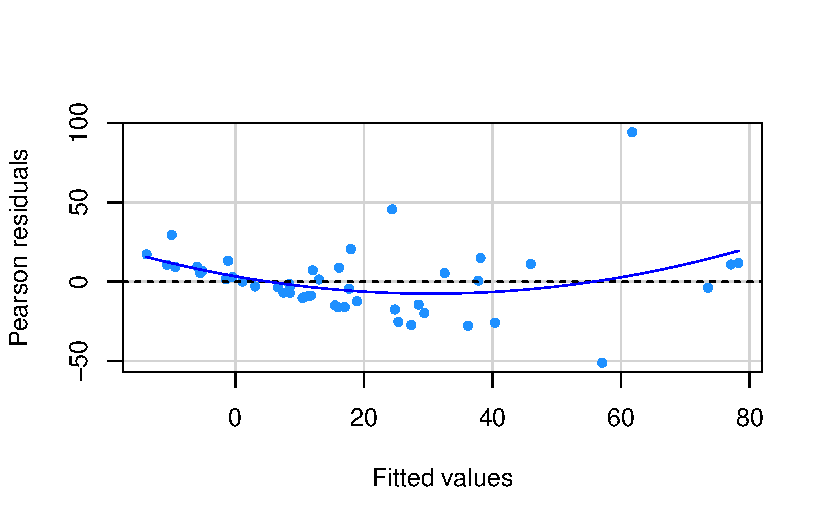
\includegraphics[keepaspectratio]{HW7_files/figure-pdf/unnamed-chunk-4-1.pdf}}

\begin{verbatim}
           Test stat Pr(>|Test stat|)   
Tukey test    2.7242         0.006445 **
---
Signif. codes:  0 '***' 0.001 '**' 0.01 '*' 0.05 '.' 0.1 ' ' 1
\end{verbatim}

\begin{itemize}
\item
  1.B. Check the constant error variance assumption using both residual
  plots and a formal statistical test. What do you conclude?

  \begin{itemize}
  \tightlist
  \item
    We further examine the constant variance assumption by plotting
    squared root of the residuals against fitted values and it seems
    that we have non-constant variance based on the plot below.
    Numerically we take note of a weak correlation between the residuals
    and predictors, but when we model these values we see that for every
    one unit increase in fitted values residuals increase by about .03,
    suggesting that there is evidence for non-constant variance, or
    heteroscedasticity

    \begin{itemize}
    \tightlist
    \item
      Note. in a F-test for equal variances, for fitted values equal to
      or below 30 versus above 30 we see that the variances in the
      residuals are not equal based on that the confidence intervals
      (95\% {[}.052, .414{]}) does not contain 0.
    \end{itemize}
  \end{itemize}
\end{itemize}

\begin{Shaded}
\begin{Highlighting}[]
\FunctionTok{plot}\NormalTok{(}\FunctionTok{check\_heteroskedasticity}\NormalTok{(mod))}
\end{Highlighting}
\end{Shaded}

\pandocbounded{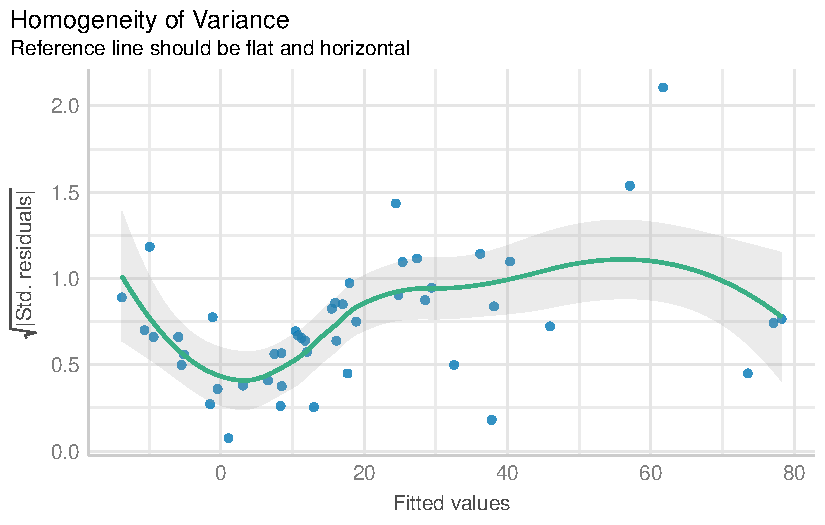
\includegraphics[keepaspectratio]{HW7_files/figure-pdf/unnamed-chunk-5-1.pdf}}

\begin{Shaded}
\begin{Highlighting}[]
\FunctionTok{cor}\NormalTok{(}\FunctionTok{fitted}\NormalTok{(mod), }\FunctionTok{resid}\NormalTok{(mod))}
\end{Highlighting}
\end{Shaded}

\begin{verbatim}
[1] 0.00000000000000002404056
\end{verbatim}

\begin{Shaded}
\begin{Highlighting}[]
\FunctionTok{summary}\NormalTok{(}\FunctionTok{lm}\NormalTok{(}\FunctionTok{sqrt}\NormalTok{(}\FunctionTok{abs}\NormalTok{(}\FunctionTok{residuals}\NormalTok{(mod))) }\SpecialCharTok{\textasciitilde{}} \FunctionTok{fitted}\NormalTok{(mod)))}
\end{Highlighting}
\end{Shaded}

\begin{verbatim}

Call:
lm(formula = sqrt(abs(residuals(mod))) ~ fitted(mod))

Residuals:
   Min     1Q Median     3Q    Max 
-3.055 -1.206 -0.072  0.733  5.176 

Coefficients:
            Estimate Std. Error t value         Pr(>|t|)    
(Intercept)  2.87838    0.31218   9.220 0.00000000000621 ***
fitted(mod)  0.02679    0.01050   2.552           0.0142 *  
---
Signif. codes:  0 '***' 0.001 '**' 0.01 '*' 0.05 '.' 0.1 ' ' 1

Residual standard error: 1.628 on 45 degrees of freedom
Multiple R-squared:  0.1265,    Adjusted R-squared:  0.107 
F-statistic: 6.514 on 1 and 45 DF,  p-value: 0.01417
\end{verbatim}

\begin{Shaded}
\begin{Highlighting}[]
\FunctionTok{var.test}\NormalTok{(}\FunctionTok{resid}\NormalTok{(mod)[}\FunctionTok{fitted}\NormalTok{(mod)}\SpecialCharTok{\textless{}=}\DecValTok{30}\NormalTok{],}
\SpecialCharTok{+}          \FunctionTok{resid}\NormalTok{(mod)[}\FunctionTok{fitted}\NormalTok{(mod)}\SpecialCharTok{\textgreater{}}\DecValTok{30}\NormalTok{])}
\end{Highlighting}
\end{Shaded}

\begin{verbatim}

    F test to compare two variances

data:  resid(mod)[fitted(mod) <= 30] and +resid(mod)[fitted(mod) > 30]
F = 0.16983, num df = 35, denom df = 10, p-value = 0.00007413
alternative hypothesis: true ratio of variances is not equal to 1
95 percent confidence interval:
 0.05178625 0.41442186
sample estimates:
ratio of variances 
         0.1698276 
\end{verbatim}

\begin{itemize}
\item
  1.C. Check the error normality assumption both graphically and
  statistically. What do you conclude? Which method do you think is
  preferable?

  \begin{itemize}
  \tightlist
  \item
    Our visuals show that the distribution of residuals are not normally
    distributed. In the density plot we see a bump emerging at the right
    tail, while our qq-plot shows several observations outside of what
    is expected.
  \item
    Additionally, we used the Shapiro-Wilk normality test and failed to
    reject the null hypothesis that the residuals are normally
    distributed in favor of the alternative hypothesis that they are
    probably not normal. We conclude that both graphically and
    statistically the assumption of error normality is violated and
    place more weight on the statistical test over our graphics.
  \end{itemize}
\end{itemize}

\begin{Shaded}
\begin{Highlighting}[]
\FunctionTok{grid.arrange}\NormalTok{(}
  \FunctionTok{plot}\NormalTok{(}\FunctionTok{check\_normality}\NormalTok{(mod), }\AttributeTok{type=}\StringTok{"density"}\NormalTok{), }
  \FunctionTok{plot}\NormalTok{(}\FunctionTok{check\_normality}\NormalTok{(mod), }\AttributeTok{type=}\StringTok{"qq"}\NormalTok{)}
\NormalTok{)}
\end{Highlighting}
\end{Shaded}

\pandocbounded{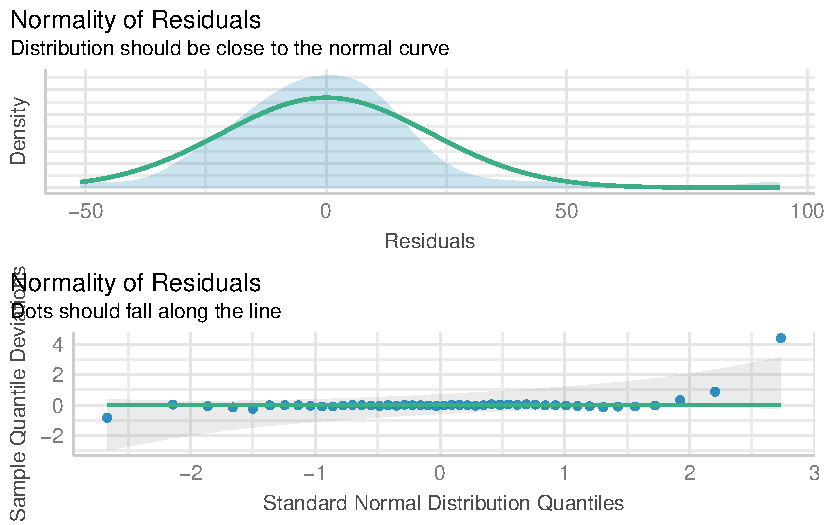
\includegraphics[keepaspectratio]{HW7_files/figure-pdf/unnamed-chunk-7-1.pdf}}

\begin{Shaded}
\begin{Highlighting}[]
\FunctionTok{shapiro.test}\NormalTok{(}\FunctionTok{resid}\NormalTok{(mod))}
\end{Highlighting}
\end{Shaded}

\begin{verbatim}

    Shapiro-Wilk normality test

data:  resid(mod)
W = 0.86839, p-value = 0.0000816
\end{verbatim}

\begin{itemize}
\item
  1.D. Check for observations with large leverage. Which observations
  have large leverage?

  \begin{itemize}
  \tightlist
  \item
    We assess the leverage H statistic using the \texttt{hatvalues()}
    function as well as plot these statistics using the
    \texttt{halfnorm()} function and find that for observations 31, 33,
    35, and 42 we may want to further investigate how these observations
    influence the model estimates.
  \item
    Recommendation: We recommend removing each one of these observations
    one by one and fitting the model, compare, residuals to determine
    how much the prediction line moves upon removing a high leveraged
    observation.
  \end{itemize}
\end{itemize}

\begin{Shaded}
\begin{Highlighting}[]
\NormalTok{hat }\OtherTok{\textless{}{-}} \FunctionTok{hatvalues}\NormalTok{(mod) }\SpecialCharTok{|\textgreater{}} 
  \FunctionTok{as.data.frame}\NormalTok{() }\SpecialCharTok{|\textgreater{}} 
  \FunctionTok{rowid\_to\_column}\NormalTok{() }\SpecialCharTok{|\textgreater{}} 
  \FunctionTok{rename}\NormalTok{(}\AttributeTok{hat=}\DecValTok{2}\NormalTok{) }\SpecialCharTok{|\textgreater{}} 
  \FunctionTok{mutate}\NormalTok{(}\AttributeTok{high\_leverage =} \FunctionTok{ifelse}\NormalTok{(hat  }\SpecialCharTok{\textgreater{}} \DecValTok{2}\SpecialCharTok{*}\FunctionTok{mean}\NormalTok{(hat), }\DecValTok{1}\NormalTok{, }\DecValTok{0}\NormalTok{)) }

\NormalTok{hat }\SpecialCharTok{|\textgreater{}} \FunctionTok{summarise}\NormalTok{(}\FunctionTok{mean}\NormalTok{(hat))}
\end{Highlighting}
\end{Shaded}

\begin{verbatim}
  mean(hat)
1  0.106383
\end{verbatim}

\begin{Shaded}
\begin{Highlighting}[]
\NormalTok{hat }\SpecialCharTok{|\textgreater{}} \FunctionTok{filter}\NormalTok{(high\_leverage}\SpecialCharTok{==}\DecValTok{1}\NormalTok{) }\SpecialCharTok{|\textgreater{}} \FunctionTok{select}\NormalTok{(}\SpecialCharTok{{-}}\NormalTok{high\_leverage)}
\end{Highlighting}
\end{Shaded}

\begin{verbatim}
  rowid       hat
1    31 0.2395031
2    33 0.2213439
3    35 0.3118029
4    42 0.3016088
\end{verbatim}

\begin{Shaded}
\begin{Highlighting}[]
\FunctionTok{halfnorm}\NormalTok{(}\FunctionTok{hatvalues}\NormalTok{(mod))}
\end{Highlighting}
\end{Shaded}

\pandocbounded{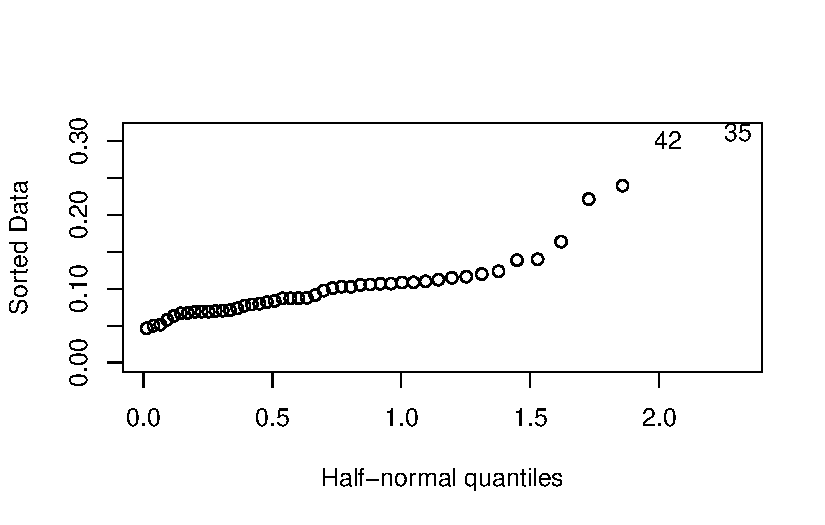
\includegraphics[keepaspectratio]{HW7_files/figure-pdf/unnamed-chunk-9-1.pdf}}

\begin{itemize}
\item
  1.E. Check for outliers. List any potential outliers.

  \begin{itemize}
  \tightlist
  \item
    Using studentized residuals, any residual divided by its error if
    greater than 3, we determine that observation 24 is an outlier. We
    further examine a boxplot for raw gambling scores and take note that
    observation 24 is far away from the mean.

    \begin{itemize}
    \tightlist
    \item
      Note. Given that we test every observation, we make a Bonferroni
      correction test by adjusting the critical value.
    \end{itemize}
  \item
    Recommendation: We recommend removing observation 24 as it is a
    potential outlier and refitting the model.
  \end{itemize}
\end{itemize}

\begin{Shaded}
\begin{Highlighting}[]
\NormalTok{r\_it }\OtherTok{\textless{}{-}} \FunctionTok{rstandard}\NormalTok{(mod) }\SpecialCharTok{|\textgreater{}} 
  \FunctionTok{as.data.frame}\NormalTok{() }\SpecialCharTok{|\textgreater{}} 
  \FunctionTok{rowid\_to\_column}\NormalTok{() }\SpecialCharTok{|\textgreater{}} 
  \FunctionTok{rename}\NormalTok{(}\AttributeTok{stud\_resid =} \DecValTok{2}\NormalTok{) }\SpecialCharTok{|\textgreater{}} 
  \FunctionTok{mutate}\NormalTok{(}\AttributeTok{outlier =} \FunctionTok{ifelse}\NormalTok{(}
    \FunctionTok{abs}\NormalTok{(stud\_resid) }\SpecialCharTok{\textgreater{}} \FunctionTok{qt}\NormalTok{(}\DecValTok{1}\FloatTok{{-}.05}\SpecialCharTok{/} \FunctionTok{n}\NormalTok{(),}\FunctionTok{n}\NormalTok{()}\SpecialCharTok{{-}}\DecValTok{2}\NormalTok{), }\DecValTok{1}\NormalTok{, }\DecValTok{0}\NormalTok{))}

\NormalTok{r\_it }\SpecialCharTok{|\textgreater{}} \FunctionTok{filter}\NormalTok{(outlier }\SpecialCharTok{==} \DecValTok{1}\NormalTok{) }\SpecialCharTok{|\textgreater{}} \FunctionTok{select}\NormalTok{(}\SpecialCharTok{{-}}\NormalTok{outlier)}
\end{Highlighting}
\end{Shaded}

\begin{verbatim}
  rowid stud_resid
1    24    4.43762
\end{verbatim}

\begin{Shaded}
\begin{Highlighting}[]
\FunctionTok{Boxplot}\NormalTok{(teengamb}\SpecialCharTok{$}\NormalTok{gamble)}
\end{Highlighting}
\end{Shaded}

\pandocbounded{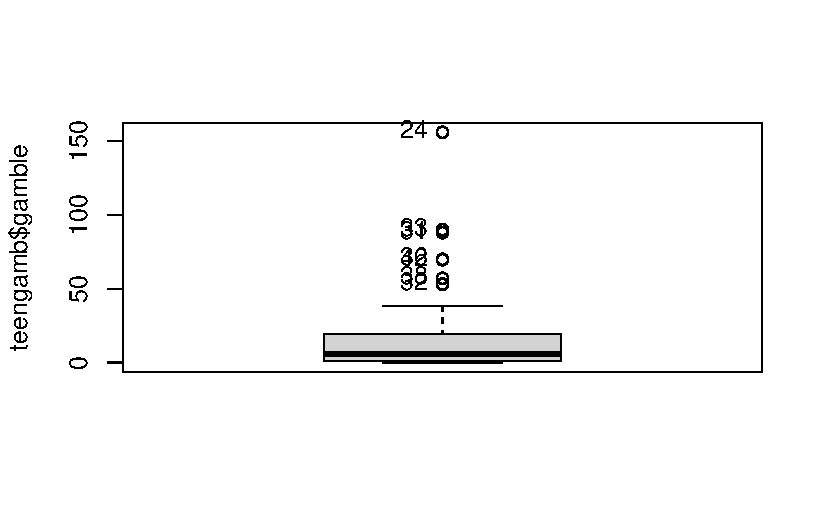
\includegraphics[keepaspectratio]{HW7_files/figure-pdf/unnamed-chunk-10-1.pdf}}

\begin{verbatim}
[1] 24 31 32 33 36 38 42
\end{verbatim}

\begin{itemize}
\item
  1.F. Check for influential points. List any potential influential
  points.

  \begin{itemize}
  \tightlist
  \item
    We use Cooks statistic to identify any influential observations and
    again find observation 24 to be problematic as seen in the halfnorm
    plot.
  \item
    Recommendation: We recommend removing observation 24 as it is a
    potential outlier and influential value and refitting the model.
  \end{itemize}
\end{itemize}

\begin{Shaded}
\begin{Highlighting}[]
\NormalTok{cd}\OtherTok{\textless{}{-}}\FunctionTok{cooks.distance}\NormalTok{(mod)}

\FunctionTok{summary}\NormalTok{(cd)}
\end{Highlighting}
\end{Shaded}

\begin{verbatim}
     Min.   1st Qu.    Median      Mean   3rd Qu.      Max. 
0.0000007 0.0011908 0.0048478 0.0248308 0.0155806 0.5565011 
\end{verbatim}

\begin{Shaded}
\begin{Highlighting}[]
\FunctionTok{halfnorm}\NormalTok{(cd)}
\end{Highlighting}
\end{Shaded}

\pandocbounded{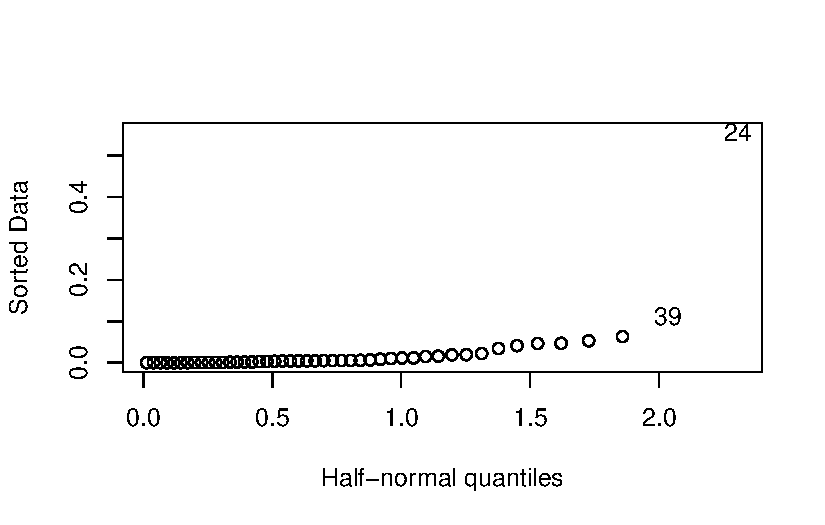
\includegraphics[keepaspectratio]{HW7_files/figure-pdf/unnamed-chunk-11-1.pdf}}

\begin{itemize}
\tightlist
\item
  We can also use the car package to see how well our assessment of high
  leverage, outliers, and influential observations we did. We find that
  we overlap in identifying 24, 42, and 35, but not 31 or 33 due to high
  hat values. In the car assessment we also see that 39 gets flagged;
  however, we did not identify this as a problem given a low studentized
  residual.

  \begin{itemize}
  \tightlist
  \item
    Note. in the plot below we take note that observation 24 has a high
    cook statistic as well as a high studentized residual despite having
    a low hat value.
  \end{itemize}
\end{itemize}

\begin{Shaded}
\begin{Highlighting}[]
\FunctionTok{influencePlot}\NormalTok{(mod)}
\end{Highlighting}
\end{Shaded}

\pandocbounded{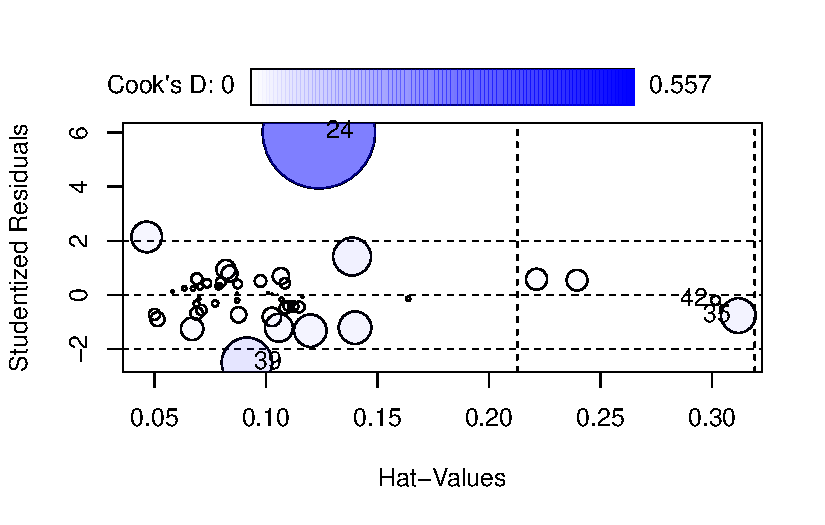
\includegraphics[keepaspectratio]{HW7_files/figure-pdf/unnamed-chunk-12-1.pdf}}

\begin{verbatim}
      StudRes        Hat      CookD
24  6.0161163 0.12380463 0.55650113
35 -0.7612557 0.31180294 0.05304304
39 -2.5060898 0.09155208 0.11244983
42 -0.1999795 0.30160877 0.00353499
\end{verbatim}

\begin{itemize}
\tightlist
\item
  1.G. Check the structure of relationship between the predictors and
  the response. What do you observe?

  \begin{itemize}
  \tightlist
  \item
    We perform partial regression subsetting by sex. We observe that the
    model subset by males has an adjusted r-squared of .50 while for
    females it was .07, although there are almost twice as many males in
    the sample.

    \begin{itemize}
    \tightlist
    \item
      talk about the differences in coefficients and confidence
      intervals.
    \end{itemize}
  \end{itemize}
\end{itemize}

\begin{Shaded}
\begin{Highlighting}[]
\NormalTok{mod\_male}\OtherTok{\textless{}{-}}\FunctionTok{lm}\NormalTok{(gamble }\SpecialCharTok{\textasciitilde{}}\NormalTok{ status }\SpecialCharTok{+}\NormalTok{ income }\SpecialCharTok{+}\NormalTok{ verbal,}
             \FunctionTok{subset}\NormalTok{(teengamb, sex }\SpecialCharTok{==} \DecValTok{0}\NormalTok{))}

\NormalTok{mod\_female}\OtherTok{\textless{}{-}}\FunctionTok{lm}\NormalTok{(gamble }\SpecialCharTok{\textasciitilde{}}\NormalTok{ status }\SpecialCharTok{+}\NormalTok{ income }\SpecialCharTok{+}\NormalTok{ verbal,}
               \FunctionTok{subset}\NormalTok{(teengamb, sex }\SpecialCharTok{==} \DecValTok{1}\NormalTok{))}

\FunctionTok{summary}\NormalTok{(mod\_male); }\FunctionTok{summary}\NormalTok{(mod\_female)}
\end{Highlighting}
\end{Shaded}

\begin{verbatim}

Call:
lm(formula = gamble ~ status + income + verbal, data = subset(teengamb, 
    sex == 0))

Residuals:
    Min      1Q  Median      3Q     Max 
-56.654 -12.104  -2.061   7.729  83.903 

Coefficients:
            Estimate Std. Error t value Pr(>|t|)    
(Intercept)  27.6354    22.2192   1.244 0.225600    
status       -0.1456     0.4181  -0.348 0.730748    
income        6.0291     1.3288   4.537 0.000135 ***
verbal       -2.9748     3.0596  -0.972 0.340617    
---
Signif. codes:  0 '***' 0.001 '**' 0.01 '*' 0.05 '.' 0.1 ' ' 1

Residual standard error: 26.45 on 24 degrees of freedom
Multiple R-squared:  0.5536,    Adjusted R-squared:  0.4977 
F-statistic: 9.919 on 3 and 24 DF,  p-value: 0.0001936
\end{verbatim}

\begin{verbatim}

Call:
lm(formula = gamble ~ status + income + verbal, data = subset(teengamb, 
    sex == 1))

Residuals:
    Min      1Q  Median      3Q     Max 
-8.6972 -2.0567 -0.5836  2.6533 11.2536 

Coefficients:
            Estimate Std. Error t value Pr(>|t|)  
(Intercept)  -5.3778     7.1848  -0.749   0.4657  
status        0.2073     0.1038   1.997   0.0643 .
income        0.6813     0.5177   1.316   0.2079  
verbal       -0.1392     0.9259  -0.150   0.8825  
---
Signif. codes:  0 '***' 0.001 '**' 0.01 '*' 0.05 '.' 0.1 ' ' 1

Residual standard error: 4.974 on 15 degrees of freedom
Multiple R-squared:  0.2228,    Adjusted R-squared:  0.06738 
F-statistic: 1.433 on 3 and 15 DF,  p-value: 0.2723
\end{verbatim}

\begin{Shaded}
\begin{Highlighting}[]
\FunctionTok{confint}\NormalTok{(mod\_male); }\FunctionTok{confint}\NormalTok{(mod\_female) }
\end{Highlighting}
\end{Shaded}

\begin{verbatim}
                 2.5 %     97.5 %
(Intercept) -18.222842 73.4936478
status       -1.008459  0.7173273
income        3.286586  8.7715717
verbal       -9.289502  3.3399831
\end{verbatim}

\begin{verbatim}
                   2.5 %    97.5 %
(Intercept) -20.69187319 9.9361899
status       -0.01396582 0.4286003
income       -0.42212178 1.7847306
verbal       -2.11265621 1.8341712
\end{verbatim}




\end{document}
